\documentclass[border=5pt]{standalone}

\usepackage{tikz}
    \usetikzlibrary{%
        arrows.meta,
        decorations.pathreplacing,
        decorations.text,
        patterns,
        shapes.arrows,
        shapes.geometric
    }

\definecolor{blue}{HTML}{0072B2}
\definecolor{green}{HTML}{009E73}
\definecolor{orange}{HTML}{D55E00}
\definecolor{pink}{HTML}{CC79A7}

\pgfdeclarelayer{background}
\pgfsetlayers{background,main}

\tikzstyle{every picture} += [remember picture]
\tikzstyle{na} = [baseline=-.5ex]

\tikzset{%
    queue/.pic={%
        code{%
            \node (rect) at (38.5mm, 10mm) {};
            \draw[thick] (0, 0) -- ++(40mm, 0) -- ++(0, 20mm) -- ++(-40mm, 0);
            \foreach \val in {0, ..., #1}{%
                \draw[thick] ([xshift=-\val*5mm] 40mm, 20mm) -- ++(0, -20mm);
            };

            \foreach \val/\lab in {0/1, 1/2, 3/c-1, 4/c}{%
                \node[draw, circle, thick, minimum size=10.5mm] (\lab)
                    at (55.25mm, 30mm - \val * 10.5mm) {\footnotesize$\lab$};
                \draw[-latex, thick] (rect.east) -- (\lab.west);
            };
            
            \node at (55.25mm, 10mm) {$\vdots$};
            \node at (5mm, 10mm) {$\cdots$};
        };
    }
}

\begin{document}

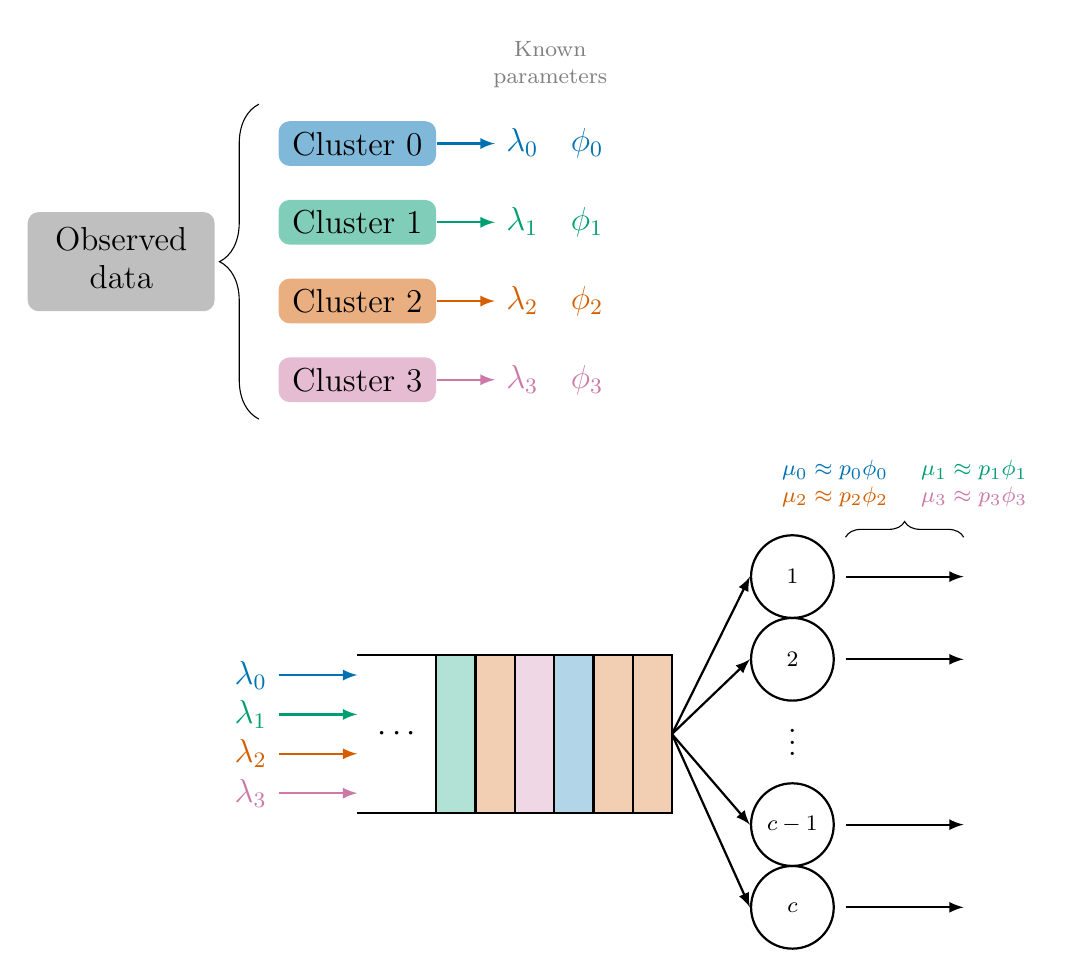
\begin{tikzpicture}

    \large%

    %%%%%%%%%%%%
    % Data
    \node[fill=gray!50, minimum width=20mm, rounded corners] (obs) at (-3, 7)
        {%
            \begin{tabular}{c}
                Observed\\
                data
            \end{tabular}
        };

    \draw[decorate, decoration={brace, amplitude=5mm}] (-1.25, 5) -- (-1.25, 9);

    \node[fill=blue!50, minimum width=20mm, rounded corners] (c0) at (0, 8.5)
        {Cluster 0};
    \node[fill=green!50, minimum width=20mm, rounded corners] (c1) at (0, 7.5)
        {Cluster 1};
    \node[fill=orange!50, minimum width=20mm, rounded corners] (c2) at (0, 6.5)
        {Cluster 2};
    \node[fill=pink!50, minimum width=20mm, rounded corners] (c3) at (0, 5.5)
        {Cluster 3};

    % Params
    \node at (25mm, 9.5) {%
        \footnotesize\color{gray}{%
            \begin{tabular}{c}
                Known\\
                parameters
            \end{tabular}
        }
    };
    \foreach \i/\colour/\cluster in {%
        0/blue/c0, 1/green/c1, 2/orange/c2, 3/pink/c3%
    }{%
        \node (params-\i) at ([xshift=15mm] \cluster.east)
            {\color{\colour}\(\lambda_{\i} \quad \phi_{\i}\)};
        \draw[-latex, thick, \colour] (\cluster.east) -- (params-\i);
    };

    %%%%%%%%%%%%
    % Queue
    \fill[orange!30] (30mm, 0) rectangle (40mm, 20mm);
    \fill[blue!30] (25mm, 0) rectangle (30mm, 20mm);
    \fill[pink!30] (20mm, 0) rectangle (25mm, 20mm);
    \fill[orange!30] (15mm, 0) rectangle (20mm, 20mm);
    \fill[green!30] (10mm, 0) rectangle (15mm, 20mm);

    \path (0, 0) pic {queue=6};
    \node (queue-in) at (0, 10mm) {};
    \node (queue-out) at (60mm, 10mm) {};

    % Arrivals
    \foreach \i/\colour in {0/blue, 1/green, 2/orange, 3/pink}{%
        \draw[-latex, \colour, thick]
            (-10mm, 17.5mm - \i * 5mm)
            to node[left, pos=0] {\color{\colour}\(\lambda_{\i}\)}
            ++(10mm, 0);
    };

    % Services
    \foreach \val in {0, 1, 3, 4}{%
        \draw[-latex, thick] (62mm, 30mm - \val * 10.5mm) -- ++(15mm, 0);
    };
    \draw[decorate, decoration={brace, amplitude=2mm}]
        (62mm, 35mm) -- ++(15mm, 0) node[midway, above=2mm] {%
            \footnotesize%
            \begin{tabular}{cc}
                \color{blue}{\(\mu_0 \approx p_0\phi_0\)} &
                \color{green}{\(\mu_1 \approx p_1\phi_1\)}\\
                \color{orange}{\(\mu_2 \approx p_2\phi_2\)} &
                \color{pink}{\(\mu_3 \approx p_3\phi_3\)}\\
            \end{tabular}
        };

\end{tikzpicture}

\end{document}
